\chapter{Opis projektnog zadatka}
		
		\textbf{\textit{dio 1. revizije}}\\
		
		Cilj ovog projekta je razviti programsku podršku za stvaranje web aplikacije "CookBooked" koja će
		omogućiti korisnicima razmjenu recepata za kuhanje i pečenje kolača te povezivanje i komunikaciju s autorima
		recepata. Platforma će ponuditi različit spektar mogućnosti ovisno o tome je li korisnik registriran ili nije.

		Prilikom pokretanja sustava prikazuje se izbornik recepata po kategorijama (prigoda, namirnice, zemlja podrijetla recepta).		
		
		Neregistrirani korisnici mogu \textbf{samo pregledavati} recepte temeljem kategorija.
		Neregistrirani korisnici vide sve detalje recepata (naslov, sastojci, koraci pripreme, posebne oznake...).
		Kako bi korisniku bilo omogućeno vršiti dodatne radnje (objava recepata, komentiranje recepata, spremanje recepata...),
		potrebno se prijaviti sa postojećim korisničkim računom ili registracijom kreirati novi korisnički račun.

		\textbf{
			Za kreiranje novog korisničkog računa potrebni su slijedeći podatci:
		}
		\begin{packed_item}
			\item \textit{korisničko ime}
			\item \textit{lozinka}
			\item \textit{ime}
			\item \textit{prezime}
			\item \textit{broj mobitela}
			\item \textit{email adresa}
		\end{packed_item}

		Registracijom u sustav korisniku se dodjeljuju prava klijenta, a naknadno mu se mogu dodijeliti prava
		vlasnika portala ili administratora. Registrirani korisnik može objavljivati recepte za kuhanje i pečenje,
		komentirati na ostale recepte itd.
				
		\underline{\textit{Klijent}} objavom recepta postaje njegov autor. Autori recepata mogu komunicirati s ostalim
		korisnicima vezano za svoje recepte (termin komunikacija = chat, videopozivi itd.). Klijent ima mogućnost označavanja, 
		komentiranja i spremanja recepata za buduću referencu. Također, kao dodatna mogućnost, pruža se i opcija praćenja 
		omiljenih autora (obavijesti). Klijent ima dvije vrste profila, javni i privatni. Na javnom su prikazani recepti,
		pratitelji i autori koje klijent prati; dok su na privatnom prikazane osobne informacije kojima klijent može
		upravljati.
		
		\underline{\textit{Vlasnik}} portala ima dodatne mogućnosti brisanja neželjenih recepata i/ili komentara ispod njih
		te mogućnost brisanja i/ili dodavanja novih kategorija recepata.

		\underline{\textit{Administrator}} sustava ima najveće ovlasti. On ima pristup bazi s popisom registriranih korisnika
		te ima mogućnost brisanja ili promijene korisničkih podataka. Također, ima svu funkcionalnost vlasnika restorana.
		
		\bigskip

		\textbf{Postojeća slična rješenja:}

		\url{https://www.coolinarika.com/}

		\begin{figure}[H]
			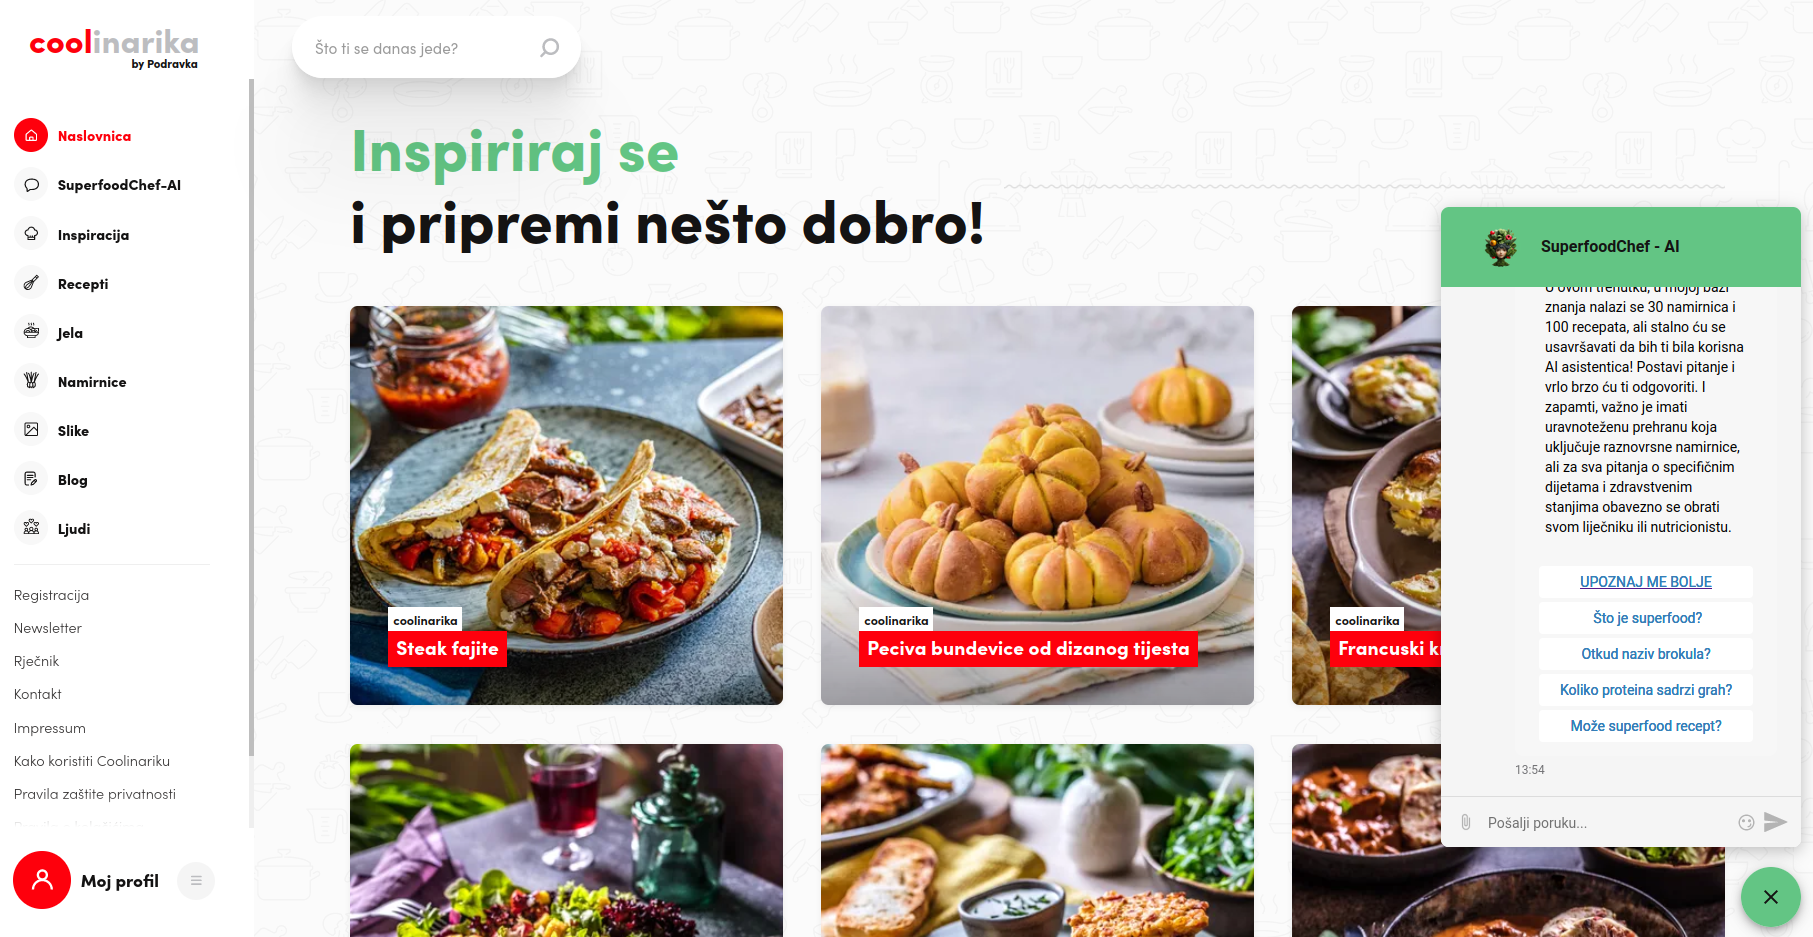
\includegraphics[scale=0.2]{slike/coolinarika.png}
			\centering
			\caption{Izgled coolinarika web portala}
			\label{fig:coolinarika}
		\end{figure}

		\url{https://recepti.index.hr/}

		\begin{figure}[H]
			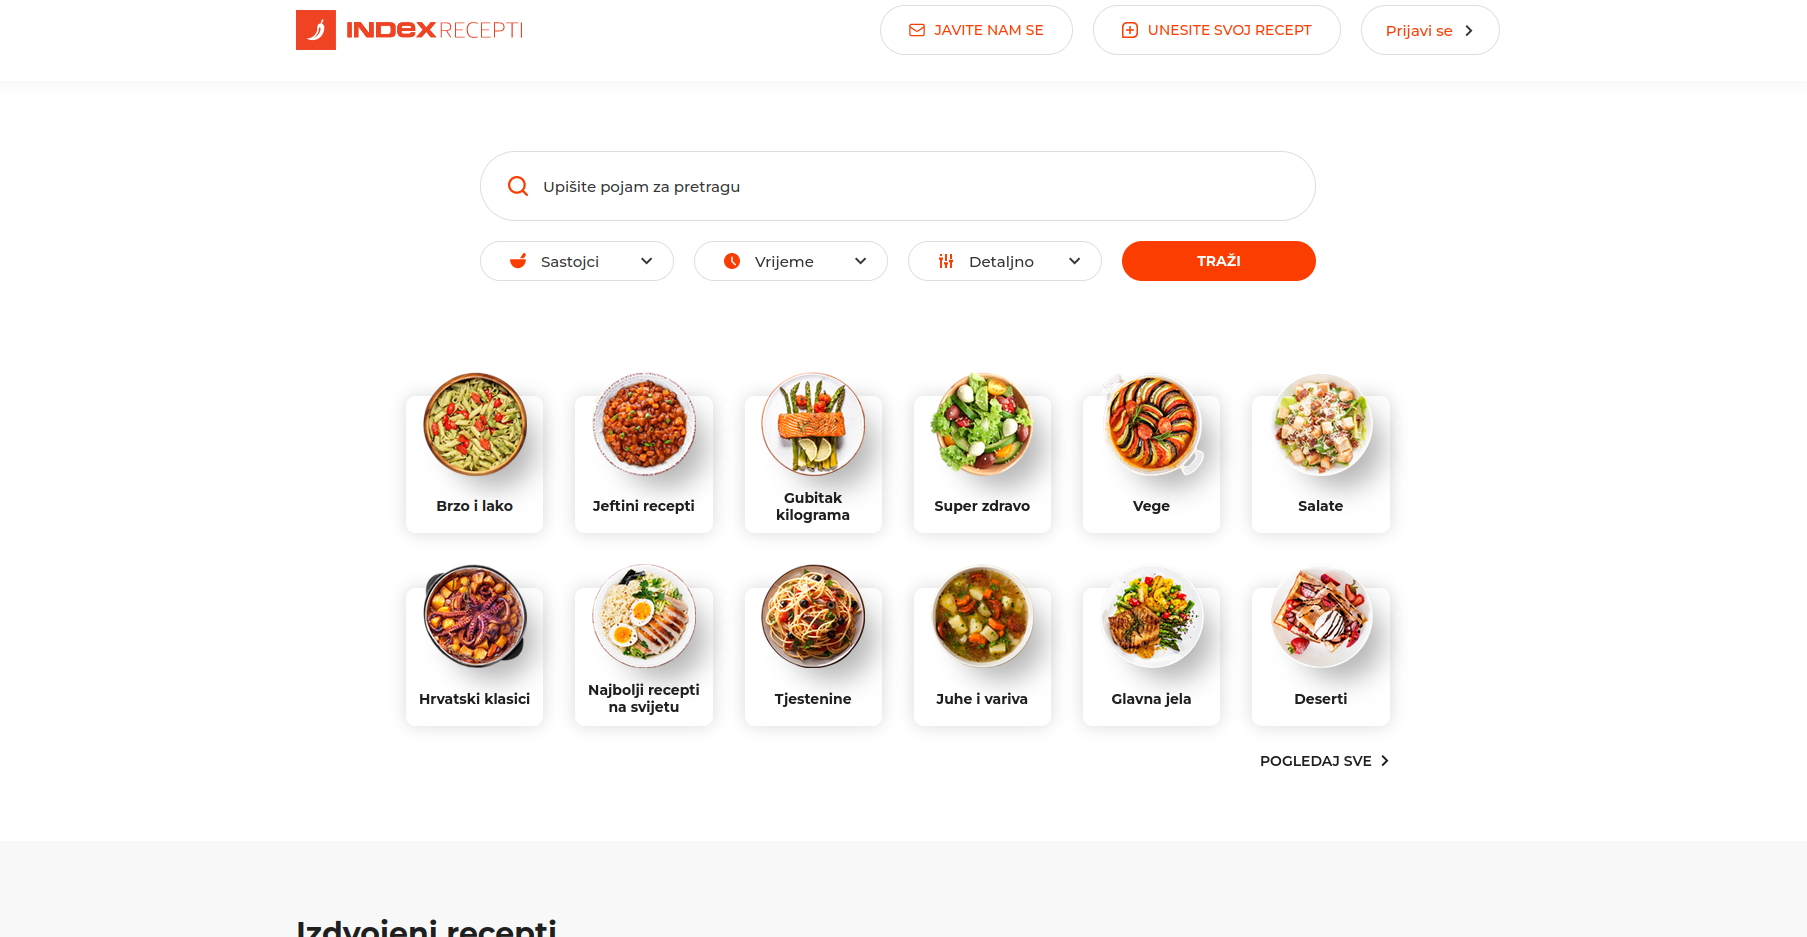
\includegraphics[scale=0.2]{slike/index-recepti.png} 
			\centering
			\caption{Izgled index-recepti web portala}
			\label{fig:index-recepti}
		\end{figure}

		\bigskip
		\bigskip
		\bigskip

		Postojeća rješenja baziraju se na proširenoj funkcionalnosti (osim kolača nude i recepte ostalih jela).
		Coolinarika nudi i dodatnu funckionalost razgovora sa AI ChatBot-om koji pomaže ljudima oko generalnog
		pojma prehrane. Također, Coolinarika ima i blog te pregled svojstava namirnica koje se koriste u receptima.

		\bigskip

		\textbf{Mogućnost nadogradnje web portala CookBooked:}

		Web portal CookBooked primarno je zamišljen kao pomoćnik u kuhanju i pečenju kolača.
		Kao takav, usmjeren je na korisnike čiji je primarni interes područje slastica.

		\smallskip

		Svaka nadogradnja postojećeg portala morala bi biti dobro iskomunicirana sa postojećim klijentima.

		\smallskip

		Mogućnosti nadogradnje:
		
		\begin{packed_item}
			\item \textit{dodavanje recepata koji nisu vezani za kolače}
			\item \textit{prijenos uživo pripremanja recepata}
			\item \textit{dodavanje oglasnik poslova vezanih uz kulinarstvo/slastičarstvo}
			\item \textit{dodavanje premium sadržaja dostupnog samo plaćenim klijentima}
		\end{packed_item}

		\textbf{Financiranje web portala CookBooked:}

		Održavanje i nadogradnja web portala CookBooked planiraju se financirati iz slijedećih izvora:

		\begin{packed_item}
			\item \textit{plaćeni oglasi na web portalu}
			\item \textit{prodaja premium korisničkih mogućnosti (u planu)}
			\item \textit{donacije}
		\end{packed_item}




		\eject
		
	